\documentclass[a4paper]{article}
\usepackage[UTF8]{ctex}
\usepackage{geometry}
\usepackage{graphicx}
\usepackage{url}
\usepackage{multirow}
\usepackage{array}
\usepackage{booktabs}
\usepackage{url}
\usepackage{enumitem}
\usepackage{graphicx}
\usepackage{float}
\usepackage{amssymb}
\usepackage{amsmath}
\usepackage{subfig}
\usepackage{longtable}
\usepackage{pifont}
\usepackage{color}

\allowdisplaybreaks

\geometry{a4paper, scale=0.78}

% \begin{figure}[H]
%     \centering
%     \includegraphics[width=.55\textwidth]{E.png}
%     \caption{矩阵与列向量的乘法}
%     \label{fig:my_label_1}
% \end{figure}

% \left\{
% \begin{array}{ll}
%       x+2x+z=2 & \\
%       3x+8y+z=12 & \\
%       4y+z=2
% \end{array}
% \right.

% \begin{enumerate}[itemindent = 1em, itemsep = 0.4pt, parsep=0.5pt, topsep = 0.5pt]

% \end{enumerate}

%\stackrel{a}{\longrightarrow}

%\underbrace{}_{} %下括号

\title{Markov Chain Monte Carlo 02 Markov Chain}
\author{Chen Gong}
\date{31 December 2019}

\begin{document}
\maketitle
在上一小节中,我们描述了三种采样方法,也就是概率分布采样法,拒绝采样法和重要性采样法。这三种采样方法在高维情况下的采样效率很低,所以我们需要另找方法。
\section{基础概念介绍}
首先我们要明确什么是Random Process,也就是它研究的变量是一个随机变量的序列$\{x_t\}$。通俗的说就是,随机过程就是一个序列,而这个序列中的每一个元素都是一个随机变量。

而Markov Chain就是一个特殊的随机过程,它的时间和状态都是离散的。并且,Markov Chain需要满足Markov性质,也就是未来和过去是无关的。我们用数学的语言表达就是:
\begin{equation}
    P(x_{t+1}=x|x_1,x_2,\cdots,x_t) = P(x_{t+1}|x_1,x_2,\cdots,x_{t-m})
\end{equation}

上述公式就是一个$m$阶马尔可夫性质。当$m=0$时,我们就得到了齐次(一阶)马尔可夫链,也就是满足:
\begin{equation}
    P(x_{t+1}=x|x_1,x_2,\cdots,x_t) = P(x_{t+1}|x_{t})
\end{equation}

而$P(x_{t+1}|x_{t})$这个概率我们用什么来表达呢?我们定义$\mathcal{P}$为一个转移矩阵$[P_{ij}]$,而$P_{ij} = P(x_{t+1}=j|x_t=i)$。

\section{平稳分布(Stationary Distribution)}
一个Markov Chain可以用下图来表示:
\begin{figure}[H]
    \centering
    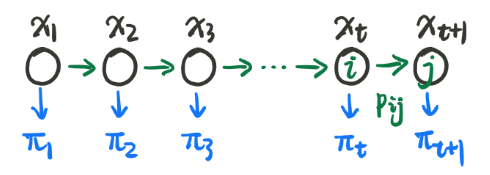
\includegraphics[width=.55\textwidth]{微信图片_20191231110648.png}
    \caption{Markov Chain Model示意图}
    \label{fig:my_label_1}
\end{figure}

此图就是一个时间序列,$x_i$就表示在第$i$时刻的状态,而每一个状态都是一个随机变量。而$\pi_i$描述的就是第$i$个随机变量的分布。对于一个马氏链来讲,它在第$t+1$时刻的概率分布,可以被我们表达为:
\begin{equation}
    \pi_{t+1}(x^\ast) = \int \pi_t(x)\cdot P(x\mapsto x^\ast) dx
\end{equation}

熟悉强化学习的同学就会觉得这个公式非常的熟悉。通俗的讲,他实际上就是在$t+1$时刻所有可能转移到状态$x^\ast$的概率的和。那么什么是随机分布呢?

假如这里存在一个$\pi$,这里的$\pi$和前面的$\pi_{t}$和$\pi_{t+1}$都没有一毛钱关系。假如$\pi$是一个概率分布,那么它可以被我们写成一个无限维向量的形式:
\begin{equation}
    \pi = [\pi(1),\pi(2),\cdots,\pi(t),\cdots], \qquad \sum_{i=1}^\infty \pi(i) = 1
\end{equation}

如果存在式(4)使得公式成立:
\begin{equation}
    \pi(x^\ast) = \int \pi(x)\cdot P(x\mapsto x^\ast) dx
\end{equation}

我们就称$\{ \pi(k) \}_{k=1}^\infty $是马氏链$\{x_{k}\}$的平稳分布。看了数学的描述我相信大部分同学还是不懂这个平稳分布时是个什么东西?用通俗的话讲就是,对于一个马氏链来说,每个时刻都符合一个概率分布,如果每一个时刻的概率的分布都是一样的都是$\pi(k)$,那么我们就可以称这个马氏链满足一个平稳分布。

那么下一个问题就是我们为什么要引入平稳分布呢?其实,我们想要去求的这个$P(Z)$,可以被我们看成是一个平稳分布$\pi(k)$,那么我们就可以通过构建一系列的$\{ x_1,x_2,\cdots,x_t,\cdots \}$的马氏链,让它来逼近这个平稳分布。那么我们构建这样的一个马氏链,包括随机变量和转移矩阵,如果它满足平稳分布的条件,确实是可以收敛到平稳分布的。那么,我就可以让构建出来的这个马氏链收敛到平稳分布来求得$P(Z)$。

既然,已经知道了什么是平稳分布了,那么下一个问题就是,我们需要知道什么样的分布可以称为平稳分布,也就是我们怎样才能构建出一个马氏链让它收敛到一个平稳分布。这里我们需要引入一个条件,也就是Detailed Balance:
\begin{equation}
    \pi(x)\cdot P(x\mapsto x^\ast) = \pi(x^\ast)\cdot P(x^\ast \mapsto x)
\end{equation}

大家直观的来想想这个公式,为什么满足它就满足了是一个平稳分布呢?其实并不难想到,对于任意两个状态之间,使用概率分布称为转移概率得到的结果都是可逆的,那么这两个状态之间的分布一定是一样的。而说如果一个分布,满足Detailed Balance那么它一定可以是一个平稳分布,但是反过来并不能成立。而证明过程也不难,如下所示:
\begin{equation}
    \begin{split}
        \int \pi(x)\cdot P(x\mapsto x^\ast)dx 
        = & \int \pi(x^\ast)\cdot P(x^\ast \mapsto x) dx \\ 
        = & \pi(x^\ast) \underbrace{\int P(x^\ast \mapsto x)}_{\sum_{j=1}^\infty P_{ij} = 1 } dx \\
        = & \pi(x^\ast)
    \end{split}
\end{equation}

这样的话,我们就可以吧不用从定义上来证明一个随机过程是马尔可夫链,直接看它满不满足Detailed Balance就可以了。而且这个公式中,$\pi$是平稳分布,$P(x\mapsto x^\ast)$是马尔可夫链的状态转移概率,这样就成功的将平稳分布和马尔可夫链结合在了一起。


\end{document}
